
A mikrovezérlős rendszerek manapság az életünk minden részében megtalálhatóak, kis méretük, 
alacsony áruk és meglehetősen nagy teljesítményükkel sok mindenre általánosan használhatóak. 
Ez nagyban csökkenti a tervezési költségeket, mivel nem kell egy specifikus logikai áramkört 
kialakítani minden egyes alkalmazási területre, csupán új program kódot kell feltölteni és 
használható egy teljesen más célra.

A mikrovezérlő könnyen összeköthetőek külső eszközökkel amellyel rengeteg mindent meg lehet 
valósítani és bővíteni a lehetőség és szabadon vezérelhetők a GPIO-n (General Purpose Input 
Output) keresztül sok mindent el lehet érni, az egyszerű LED kapcsolgatásától komplex jelek 
generálásáig. Általános esetben a mikrovezérlők csak a legfontosabb részeket tartalmazzák, 
mint az Analog Digital Converter amivel egy analóg jelet alakít egy digitális jellé amit a 
processzor fel tud majd dolgozni, ez legfőképpen azért van, mert nem mindenkinek van szüksége 
mindenre így akinek szüksége van az egyszerűen az külsőleg csatolja hozzá. 

Az összeállított rendszert szabadon lehet vezérelni így automatizálni lehet vele folyamatokat 
amivel egyszerűsíti az emberek dolgát. Viszont nagyban gyorsítja a folyamatok sebességét és 
pontosságát, miközben csökkenti a költségeket, mivel nem kell egy képzett dolgozó irányítsa, 
egy ilyen példa a robotkarok irányítása, lehetséges lenne karok segítségével irányítani, 
viszont ez lassú és költséges, mivel minden robotkar mellé kellene egy munkás aki közel sem 
lenne elég nagy pontosságú. 

Ezen kívül gyakran használják automatizált tesztelésekre is, mivel egyszerű megismételhető 
teszteket végezni velük, miközben képesek valós időben mérni a rendszer viselkedését. Ennek 
a feladatnak is ez a lényege, az alkatrészek tesztelése egy gyors és automatizált módon. 


\section{Téma meghatározása}

A dolgozat célja egy olyan eszköz tervezése, amit bárki elektronikai ismeret nélkül is egyszerűen 
használni lehet. Sok esetben a feliratok az alkatrészeken nehezen látható, lekopott vagy 
egyszerűen nincs feltüntetve. Ilyen esetben sok segítséget tud nyújtani egy olyan eszköz ami 
gyorsan meg tudja határozni a komponenst és a lábkiosztását is amennyiben ez fontos.

Ez különösen nagy segítséget nyújt kezdőknek akik még kevésbé ismerik az alkatrészeket és az 
adatlapjai meg nagyok és komplexek számukra és a fő információk megjelenítése néhány sorban. 
Haladóknak is nagy segítség, mivel az ellenállást színkódjátról egyszerű meghatározni, viszont 
a teszterrel meg lehet határozni, hogy az alkatrész hibás-e, vagyis ha a tranzisztor kiégett 
akkor az is letesztelhető.

A teszternek 3 teszt terminálja van, ebbe kell az ismeretlen komponenst bekötni és képes 
egyszerű elektronikai komponensek (ellenállás, dióda, tranzisztorok, stb.) automatikus 
felismerését és az adatainak meghatározására. Viszont nem képes bonyolultabb áramkörök 
azonosítására aminek összesen tübb mint 3 lába van.

Megvalósítás során a költégek csökkentése a cél, miközben a pontosság nem csökken nagyban. 
Két verzió is összeállítható, az egyik egyszerű ellenállásokkal és a második egy DAC (Digital 
Analog Converter) segítségével. Mindkettő alkalmas a komponensek meghatározására, viszont az 
ellenállásos verzió nem alkalmas karakterisztika diagram kirajzolására, viszont sokkal olcsóbb, 
mivel nem használ egy külső DAC-ot.

Mérés eredménye kikerül egy kis kijelzőre és grafikus felületen is megtekinthető amennyiben 
egy számítógéphez van csatolva. Viszont a 2 közül legalább az egyikre szükség van, különben a 
mérés eredménye nem lesz látható. A kijelzőt nem kötelező alkalmazni, viszont annélkül csak 
egy laptop/számítógéphez kapcsolva lehet használni.

Ehhez szükséges egy processzor, viszont manapság a mikrovezérlők nagy számítási kapacitással 
rendelkeznek meglehetősen alacsony áron és néhány ellemállásból és vezetékből otthon is 
összeállítható.

Karakterisztika diagramm kirajzolása is fontos, viszont ez leginkább a tranzisztoroknál 
fontos, mivel az ellenállások lineárins összefüggést mutatnak a feszültség és áramerősség közt 
és a diódák meg magas áram növekedést ami után a feszültésg elérte a nyitó feszültséget.

A rendszer táplálása bármilyen USB csatlakozón keresztül lehetséges, mivel ez széles körben 
megtatlálható vagy külső akkumulátor is megfelel amelynek van USB kimenete.

\section{Hasonló eszközök}

Egy hasonló rendszer már megvalósult \cite{similarSystem} ami egy Arduino\cite{ArduinoAtmega} 
mikroprocesszoron alapul. Ez egy egyszerűbb rendszer, ami csupán ellenállásokat használ az 
alkatrészek felismerésére és egy kijelzőt az adatok megjelenítésére. Ebből több fejlesztés is 
kialakult, több minden tesztelésére és nagyobb pontosság elérésére, miközben a rendszer 
egyszerűségét fenntartani. Ezek a rendszerek viszont nem használnak DAC-ot és ezért nem képesek 
karakterisztika diagramot készíteni. Ezen kívül nem csatlakoztatható egyszerűen számítógéphez, 
csupán újraprogramozás céljából, így minden esetben kell tartalmazzanak egy kijelzőt, ami 
növeli a költségeket. Az általános működésük hasonló, mint ebben a projektben, viszont itt 
precízen lehet változtatni a feszültséget, nem csak kapcsolni földre vagy tápfeszültségre.
Az bekötése hasonlóképpen történik: lásd \ref{fig:basicTesterConnection}

Mindegyik GPIO pin lehet csatolva földre, vagy tápfeszültségre, de le is lehet kapcsolva, így 
nem befolyásolja az áramkör működését. Az ADC pin meg lehet ADC üzemmódban, ilyenkor nem befolyásolja
az áramkört, viszont lehet földre, vagy tápfeszültségre is kapcsolni, ilyen esetben port ellenállás
nélkül csatolódik az áramkörre.

\begin{figure}[H]
    \centering
    \subfigure[Eredeti teszter]{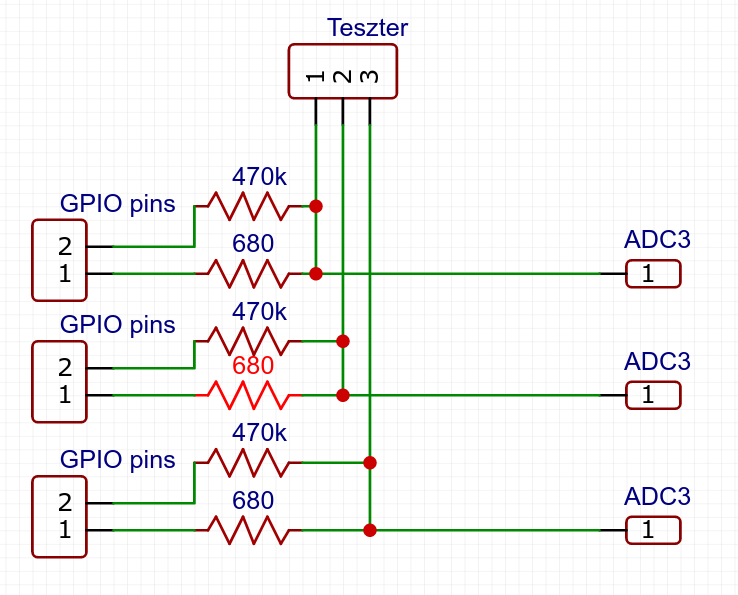
\includegraphics[scale=0.3]{figures/images/literature/OrgTesterConnection.png}}
    \caption{Eredeti teszter}
    \label{fig:basicTesterConnection}
\end{figure}